\documentclass[12pt,a4paper]{article}
\usepackage{graphicx}
\usepackage{amsmath}
\usepackage{amssymb}
\usepackage{subfigure}
\usepackage{booktabs}
\usepackage{color}
\usepackage{listings}
\usepackage{eurosym}
\usepackage{mathtools} % for \mydef
\usepackage{float}
\usepackage{natbib}
\usepackage{gensymb} % for \degree
%\usepackage{authblk} % for multiple authors with different affiliations
\usepackage[small]{titlesec}
\usepackage[displaymath, mathlines]{lineno}

% see http://tex.stackexchange.com/questions/99316/symbol-for-external-links
\usepackage{fontawesome}
\usepackage[hidelinks]{hyperref}
% Redefinition, symbol included in link:
\let\orighref\href
\renewcommand{\href}[2]{\underline{\orighref{#1}{#2}}}
% hyphens option for hyperref: enables line-breaks at hyphens. Otherwise only at slashes /. Ugly
%\PassOptionsToPackage{hyphens}{url}\usepackage{hyperref}

\addtolength{\oddsidemargin}{-2cm}
\addtolength{\evensidemargin}{-2cm}
\addtolength{\textwidth}{4cm}
\addtolength{\topmargin}{-2cm}
\addtolength{\textheight}{2cm}


\renewcommand{\familydefault}{\sfdefault}

\graphicspath{{../figures/}} 

\title{Documentation}

\author{Stefan}

%\date{}
\begin{document}
\setlength{\parindent}{0cm}
\maketitle
%\tableofcontents

% The following are interesting, but what about copyright?
%https://github.com/poidl/yassy/blob/2b6f974c33e525abc3e9d08fe0a439fb1c91d261/doc/index.html
%https://github.com/poidl/yassy/blob/2b6f974c33e525abc3e9d08fe0a439fb1c91d261/doc/filters.html

{\bf Note:} I'm a DSP beginner. The following may contain serious errors and/or be severely misleading.

\section{Postfilter for BLIT sawtooth VA synth}\label{sec:dsp}

TEst \[\frac{1}{0.65+0.35z^{-1}}\]
 I'm trying to understand the postfilter for the bandlimited sawtooth VA synth described by 
\cite[][his page 17]{frei2002digital}, defined by

\begin{equation}\label{eq:freifilter}
    \frac{1}{0.65+0.35z^{-1}}.
\end{equation}

This is an infinite impulse response (IIR) filter with a single-pole. These filters are generally of the form \citep{wiki:IIR}

\begin{equation}\label{eq:iirf}
y[n]=\frac{1}{a_0} (b_0x[n]-a_1y[n-1]).
\end{equation}

and have a transfer function defined by

\begin{equation}\label{eq:iirf_trafofct}
H(z)=\frac{b_0}{a_0+a_1z^{-1}}.
\end{equation}

Eq. \ref{eq:iirf} and \eqref{eq:iirf_trafofct} can be written in the more "traditional" \citep{wiki:IIR} forms

\begin{equation}\label{eq:iirf_normal}
y[n]=b'_0x[n]-a'_1y[n-1].
\end{equation}

and

\begin{equation}\label{eq:iirf_trafofct_normal}
H(z)=\frac{b'_0}{1+a'_1z^{-1}}
\end{equation}

by setting $b'_0=b_0/a_0$ and $a'_1=a_1/a_0$. Multiplying the previous line by $z$ yields

\begin{equation}\label{eq:iirf_trafofct_normal2}
H(z)=\frac{b'_0z}{z+a'_1},
\end{equation}

showing that $H(z)$ has a zero at $z=0$ and a pole at $z=-a'_1$. Setting $z=x+iy$ one obtains

\begin{align}
Re(H(z)) &= b'_0\frac{x^2+y^2-a'_1x}{x^2+y^2-2a'_1x+a_1^{'2}}\\
Im(H(z)) &= -\left(\frac{b'_0}{a'_1}\right)\frac{y}{x^2+y^2-2a'_1x+a_1^{'2}}.
\end{align}

The specific filter \eqref{eq:freifilter} is obtained by setting

\begin{align}
b'_0=1.54 \\
a'_1=0.54,
\end{align}

and $Re(H(z))$ is shown in Fig. \ref{fig:h}

\begin{figure}[H]
	\centering
	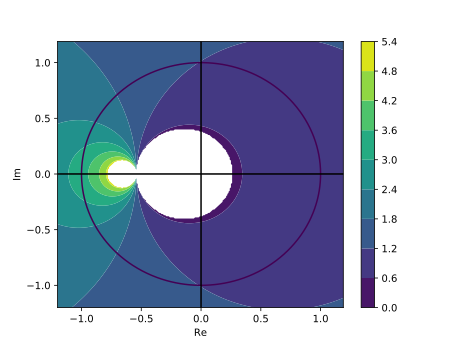
\includegraphics[width=0.8\textwidth]{h.pdf}
	\caption{$Re(H(z))$ for $a'_1=0.54$ and $b'_0=1.54$. The unit circle is shown in black.}\label{fig:h}
\end{figure}






\bibliographystyle{model2-names}
\bibliography{main.bib}
\end{document}